\section{Appendix}
\label{sec:appendix}

\subsection{Unbiasedness Regressions}
In this Appendix we build on the intuition behind the unbiasedness regressions and the measurement of market inefficiency.
We provide plots from simulated efficienct and inefficient markets, and show how the unbiasedness regressions can be used to measure the degree of inefficiency in the market.

\subsubsection{Simulated Efficient Market}
In this section we simulate an efficient market, where returns are normally distributed with a mean of 0 and a standard deviation of 0.1.
They are independent random events.

\begin{figure}[h]
    \centering
    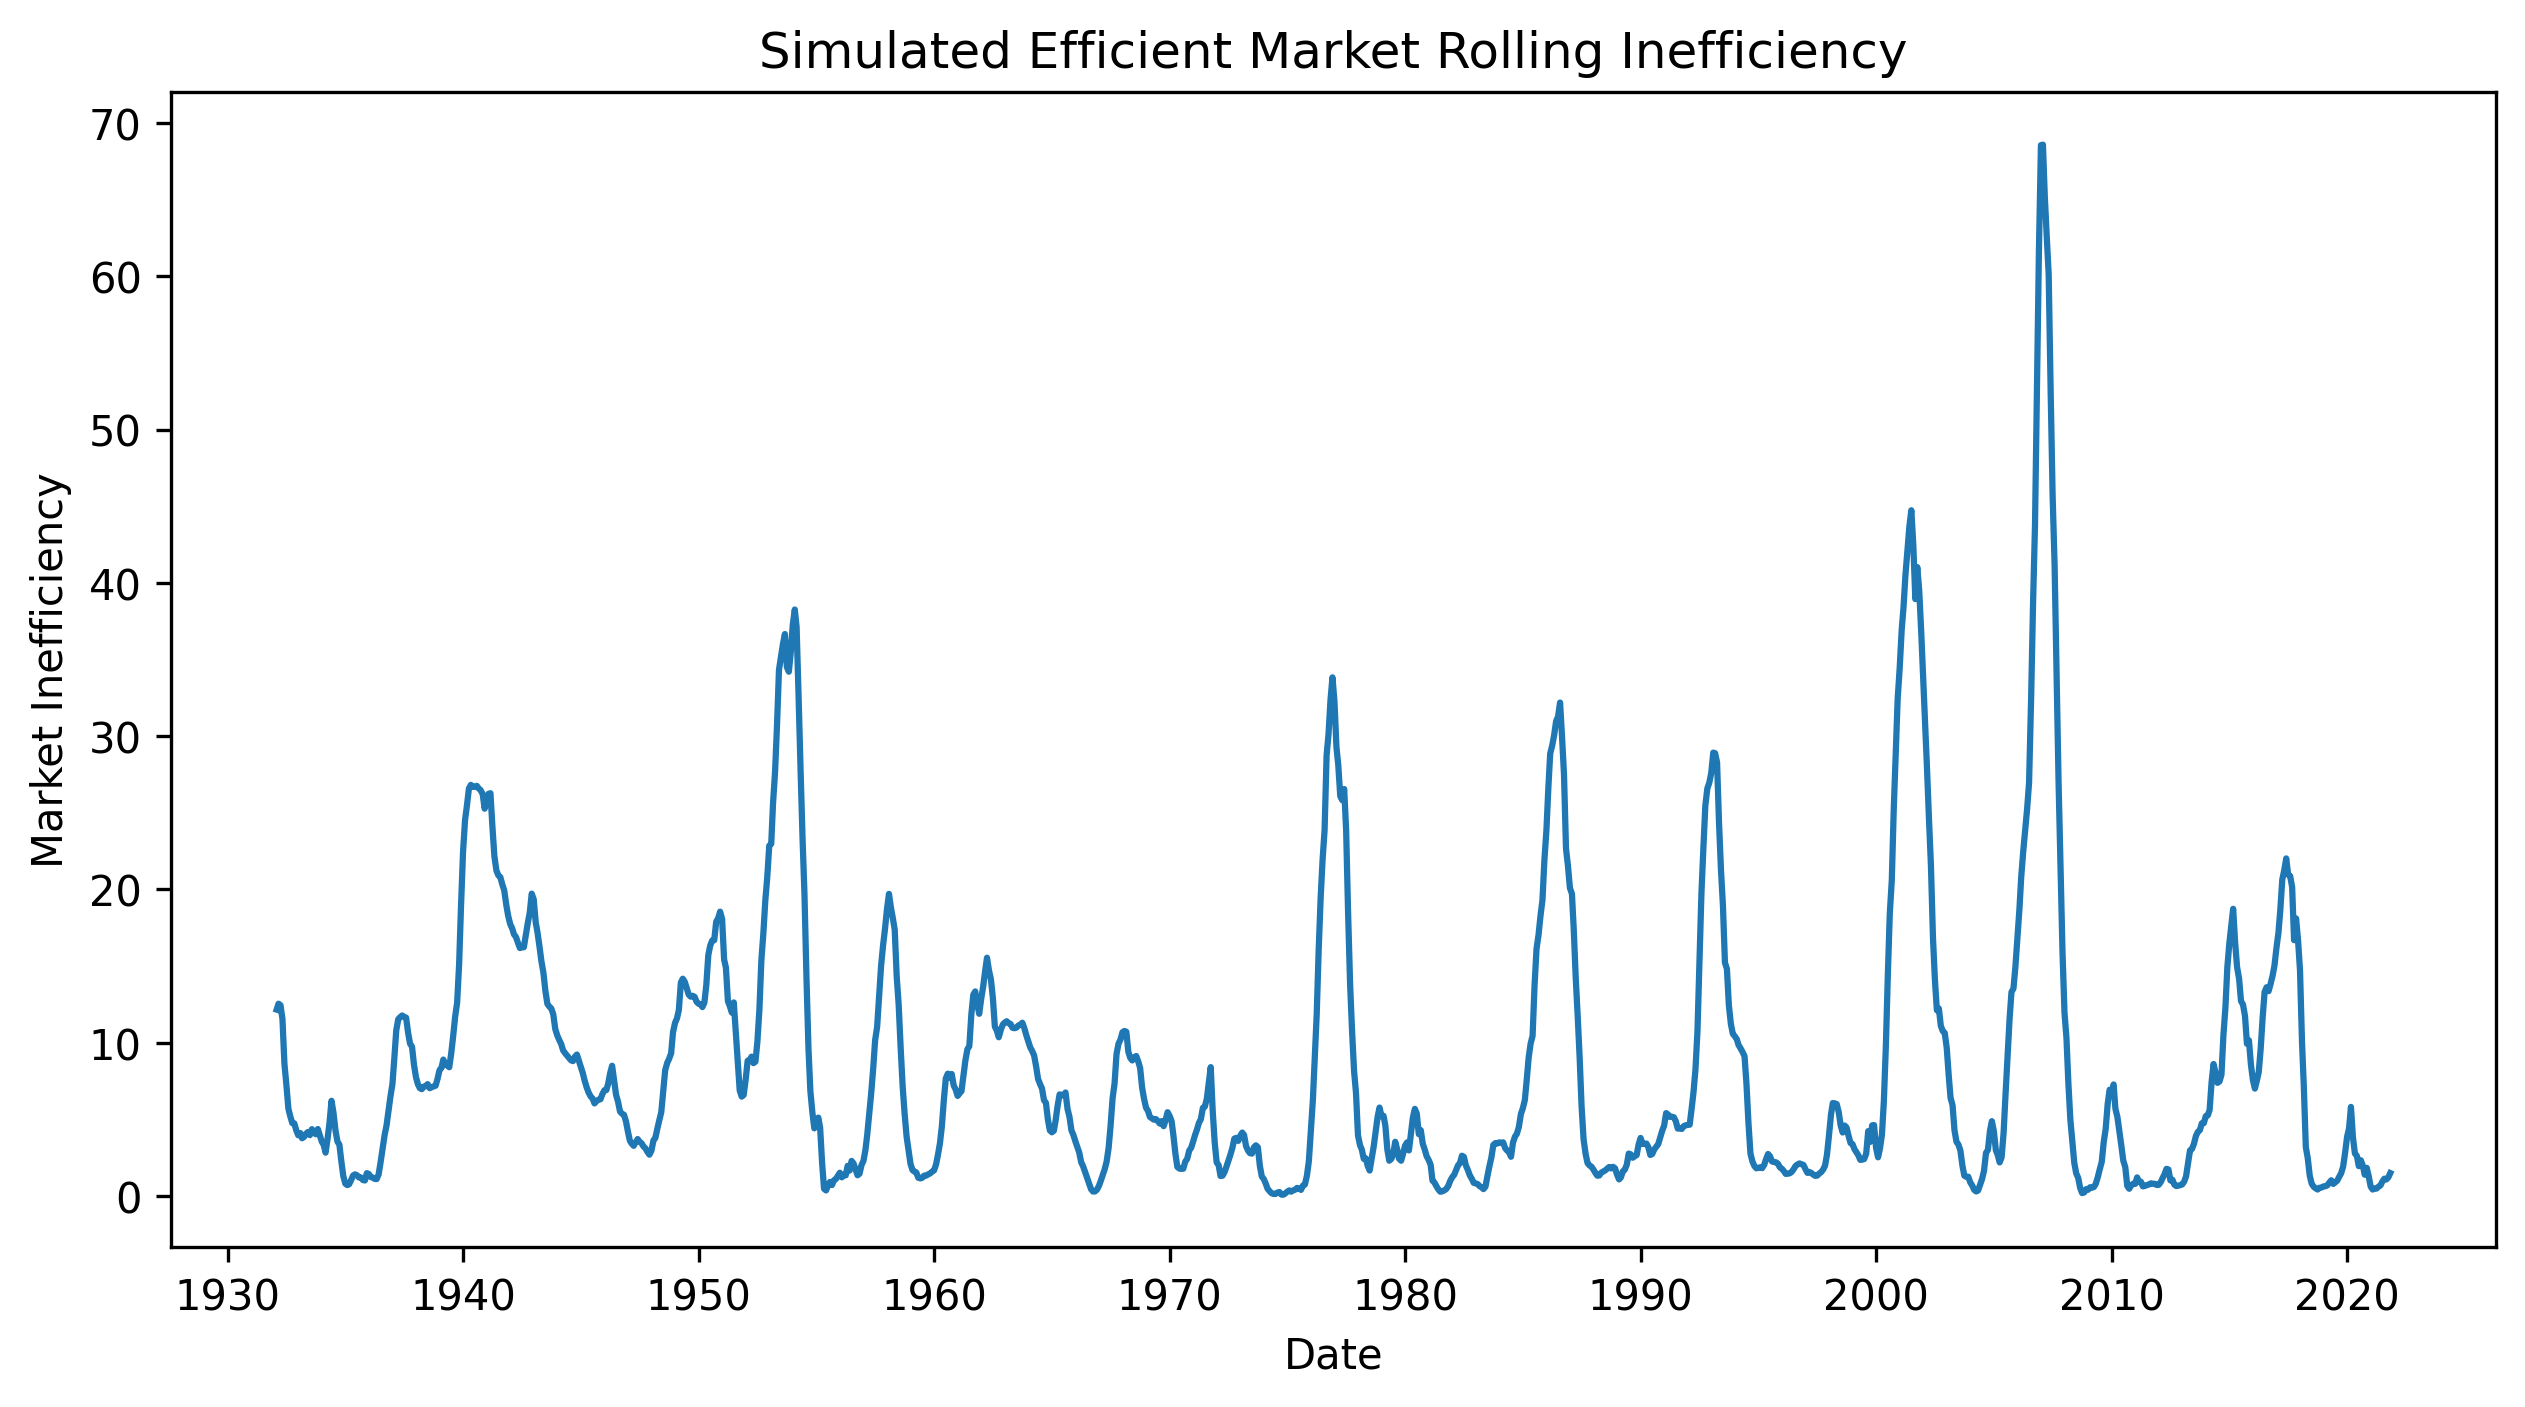
\includegraphics[width=0.8\textwidth]{../figs/Simulated Efficient Market Rolling Inefficiency.png}
    \caption{Simulated Efficient Market}
    \label{fig:efficient_market}
\end{figure}

In Figure \ref{fig:efficient_market} we see the rolling inefficiency of the simulated efficient market.
Notice that the level remains low, with only small spikes in inefficiency. There is an outlier near the end of the period
[TODO: why? just the instability of the rolling window methodology?]

\subsubsection{Simulated Inefficient Market}
In this section we simulate an inefficient market, where returns are an AR(1) process:
\begin{equation}
    r_t = \phi r_{t-1} + \epsilon_t
\end{equation}

where $\phi = 0.5$ and $\epsilon_t \sim N(0, 0.1)$. The resuling series of market inefficiency
 is shown in Figure \ref{fig:inefficient_market}. We see that there are much more frequent spikes of inefficiency, and the level of inefficiency is much higher than in the efficient market.

\begin{figure}[h]
    \centering
    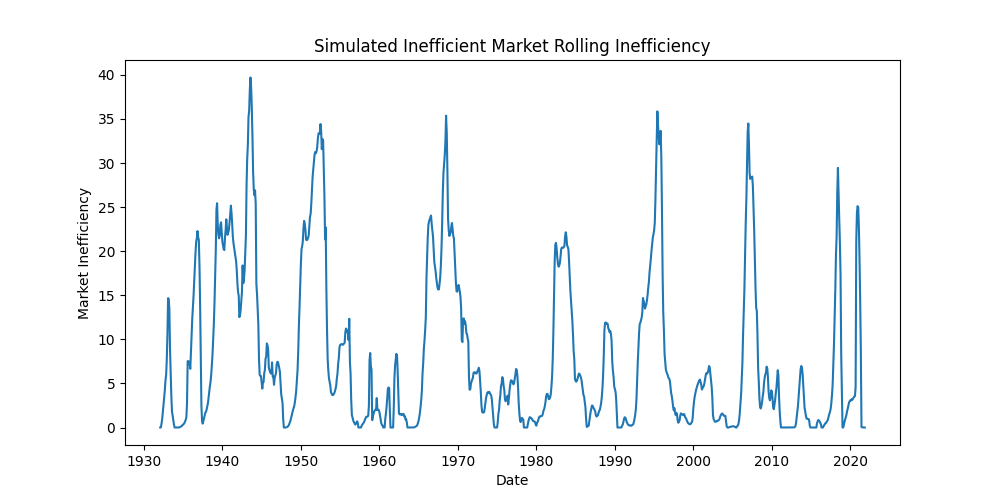
\includegraphics[width=0.8\textwidth]{../figs/Simulated Inefficient Market Rolling Inefficiency.png}
    \caption{Simulated Inefficient Market}
    \label{fig:inefficient_market}
\end{figure}
